% Fig. 3.6 -- 積空間的聯合值域如何把平面切成九塊，與 Fig. 3.7 的非積空間對照。
% 書稿來源: mathstatch3.tex 第 763 至 805 行的 tikzpicture (scale=1.15)。
%
% 幾何一律照書稿: 單位正方形值域填色、縱線 x = 1 與橫線 y = 1 把平面分成九格，
% 四個非零區塊各標一個積分式，x < 0 的左行與 y < 0 的下列共五處標 0。
%
% 對書稿的三處調整:
%   1. 填色由 gray 0.2 改為 journalaccent 0.15。
%   2. 書稿的積分式壓得較近，本圖把正方形放大並重排標示位置。
%   3. 字級: 書稿的 $f_{\sssig XY}$ 走 scriptscriptstyle 且整式加 \small，
%      在 350px 顯示寬之下最小字只有 3.0px。此處改為一般下標、去掉 \small
%      與 \displaystyle，全圖走 10pt，並以 \DeclareMathSizes 把 script 級撐到 9pt。
%      座標與版位一律取與 Fig. 3.7 相同，兩張九宮格對照圖的字因而一樣大。
%
% 量測: 見本檔同目錄的產製紀錄; 最小字 9pt，350px 顯示寬之下不得低於 11px。
%
% 產製:
%   pdflatex product-space-nine-regions.tex
%   pdftocairo -svg product-space-nine-regions.pdf ../../images/teaching-topics/product-space-nine-regions.svg

\documentclass[tikz,border=2pt]{standalone}
\usepackage{amsmath}
\usepackage{amssymb}
\usepackage{xcolor}

\definecolor{journalink}{HTML}{1F1C18}
\definecolor{journalmuted}{HTML}{8A7F72}
\definecolor{journalaccent}{HTML}{9C2D2D}

%% 下標與積分上下限一律撐到 9pt。
\DeclareMathSizes{10}{10}{9}{9}

\begin{document}
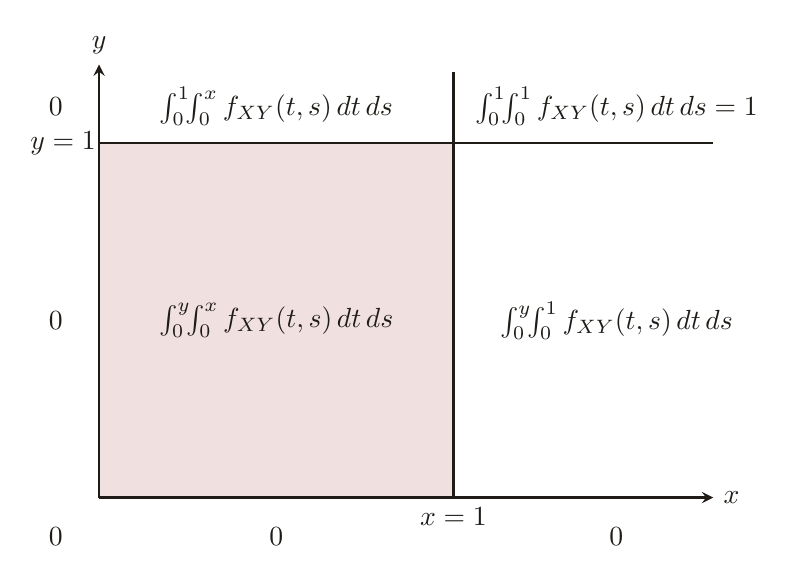
\begin{tikzpicture}[x=1cm, y=1cm, >=stealth,
                    every node/.style={journalink, font=\normalsize},
                    intg/.style={journalink, inner sep=1pt}]

  %% 聯合值域 (0,1) x (0,1) 所對應的正方形
  \fill[journalaccent, fill opacity=0.15] (1,1) rectangle (5.5,5.5);

  %% 邊界 x = 1
  \draw[journalink, line width=0.8pt] (5.5,1) -- (5.5,6.4);
  \node[journalink, below] at (5.5,1) {$x=1$};

  %% 邊界 y = 1
  \draw[journalink, line width=0.8pt] (1,5.5) -- (8.8,5.5);
  \node[journalink, left, inner sep=1pt] at (1,5.5) {$y=1$};

  %% 座標軸
  \draw[journalink, line width=0.8pt, ->] (1,1) -- (8.8,1) node[right] {$x$};
  \draw[journalink, line width=0.8pt, ->] (1,1) -- (1,6.5) node[above] {$y$};

  %% 四個非零區塊各自的積分寫法
  \node[intg] at (3.25,3.25)
    {$\int_{0}^{y}\!\!\int_{0}^{x} f_{XY}(t,s)\,dt\,ds$};
  \node[intg] at (7.57,3.25)
    {$\int_{0}^{y}\!\!\int_{0}^{1} f_{XY}(t,s)\,dt\,ds$};
  \node[intg] at (3.25,5.97)
    {$\int_{0}^{1}\!\!\int_{0}^{x} f_{XY}(t,s)\,dt\,ds$};
  \node[intg] at (7.57,5.97)
    {$\int_{0}^{1}\!\!\int_{0}^{1} f_{XY}(t,s)\,dt\,ds=1$};

  %% 其餘各區塊的 cdf 值皆為 0
  \node at (0.45,5.97) {$0$};
  \node at (0.45,3.25) {$0$};
  \node at (0.45,0.50) {$0$};
  \node at (3.25,0.50) {$0$};
  \node at (7.57,0.50) {$0$};

\end{tikzpicture}
\end{document}
